\documentclass{ecuthesis}

% Packages
\usepackage{graphicx}

% Setup the variables for the title page
\title{Using traffic analysis to identify anonymous networks}
\author{John Barker}
\department{School of Computer and Security Science}
\school{Edith Cowan University}
\degree{Computer Science (Honours)}
\email{jebarker@our.ecu.edu.au}
\studentid{0991300}
\supervisor{Dr Christopher Bolan}
\supervisor{Mr Peter Hannay}
\supervisor{Mr Patryk Szewczyk}

% Begin document
\begin{document}
\maketitle

\begin{abstract}

Traditional attacks against anonymous systems aim to uncover the identities of those involved. However, a more likely goal of attackers is to block or degrade the network itself, discouraging participation and forcing vulnerable users to communicate using less secure means. Since anonymous networks operate on known protocols and employ strong encryption it is difficult to distinguish them from regular traffic. This proposal describes a method for identifying traffic belonging to anonymous networks by examining their communication patterns.

\end{abstract}

\chapter{Introduction}

\section{Background}

The Internet has revolutionised the political sphere in providing a platform for the publication of speech to a far greater audience than was ever available before digital communications systems \citep{Bonchek:1997p3455}. The publication of less desirable political speech, criticism or challenging ideas still carries with it great risk, with numerous publications leading to arrest. This has spawned headlines such as \emph{Egypt arrests another blog critic} \citeyear{website:egypt-arrests}, \emph{Chinese couple sue Yahoo! in US over torture case} \citep{website:china-yahoo-torture}, \emph{Vietnam bloggers arrested over China shirt protest} \citep{website:vietnam-bloggers-arrested}, \emph{23 Journalists/Bloggers Arrested in Iran, Including Head of Top Group} \citeyear{website:iran-bloggers-arrested} and \emph{Blogger Arrests} \citep{website:blogger-arrests}. The Internet, like conventional media is still vulnerable to censorship by oppressive governments and malicious attackers \citep{Crandall:2007p6165,Karlin:2009p6166}.

In response to these threats, a number of systems have been proposed which use cryptography to provide censorship resistance and anonymity. Recent examples of such software include Freenet \citep{Clarke:2001p2435} and The Second Generation Onion Router (Tor). Tor is an anonymous network which uses various techniques to provide low latency anonymity to network participants \citep{Dingledine:2004p314}. It also aims to provide resistance against censorship based blocking attempts \citep{Dingledine:2008p1542}.

Although such networks provide avenues for users to avoid censorship and a certain amount of privacy, it may be possible to use traffic analysis techniques to automatically these communications and distinguish them from regular traffic. This paper proposes a quasi-experimental methodology for identifying Tor traffic which may be used by censors in the future.

\section{Significance}

Traffic analysis is a well established field, and there are a significant number of known papers that propose traffic analysis attacks against modern communications networks \citep{Zhang:2009p1188}. When considering anonymous and censorship resistant networks, typical traffic analysis attacks focus on techniques and attacks designed to uncover the identities of participants. As stated in \citet{Murdoch:2005p325} “The principal objective of an adversary attacking an anonymous communication system is to link the initiators of connections with their respective communication partners and vice versa”.

Tor’s availability, unrestrictive license and platform portability has made it a popular anonymous network with around one thousand eight hundred users at the time of writing \citep{website:tor-anonymity-online}.

The traffic analysis techniques proposed in this paper will attempt to classify network streams belonging to Tor users and distinguish them from regular encrypted communications.

\section{Research Questions}

Given a motivated and universal attacker, it is inexpensive and straightforward to disconnect a user from these networks by blocking access to well known and published resources. Once these avenues of attack have been exhausted it is still possible to connect to the network by connecting to lesser known access points. Since these networks are capable of communicating using many of the same methods as most conventional Internet applications, a blanket ban on this kind of communication would be too broad and extensive.

Tor employs strong encryption the goal of which is to ensure that the data transmitted is indistinguishable from random noise. To an observer, data transmitted using encryption looks the same. Thus the traditional means of identifying these protocols are ineffective.

This raises the question: is it possible to distinguish the traffic created by these networks, from encrypted traffic produced by conventional software? This question can be broken down further:

\begin{enumerate*}
\item Can the traffic be classified using automated matching techniques?
\item Do these networks have characteristics that make them readily distinguishable using heuristics based matching?
\item Do they have characteristics that make them distinguishable using a machine learning technique?
\item How long does a user have to be connected to the network before a confident match can be made?
\end{enumerate*}

\chapter{Literature Review}

The main areas of research included papers and proposals on the design of anonymity networks and those covering the subject of traffic analysis. Particular attention has been paid to encryption as it is the primary function by which these systems operate and a good understanding is necessary for the development of an appropriate traffic analysis method.

\section{Encryption}

Since the inception of language, hostile forces and their attempts to intercept messages have necessitated the development of secretive communications. This deliberate transformation of a messages so that only the intended recipient can understand it is known as encryption. The process of examining these obfuscated messages and attempting to reverse the transformation is known as cryptanalysis \citep{Schneier:1995p3908}. These fields have been locked in an arms race ever since, each side continually advancing their capabilities in an attempt to gain ground.

Apart from One Time Pads, no encryption methodology has ever proven to be unbreakable \citep{Shannon:2001p6583}. This means that all remaining cryptographic methods are a way of transforming information, so that for an attacker the difficulty in reversing this transformation is too costly to make it worthwhile. The invention of robots and computers was precipitated by the need to break encryption methods of increasing complexity and at the same time has lead to the increasing complexity of encryption algorithms \citep{Kahn:1967p1005}.

In \citeyear{Jevons:1874p1167}, \citeauthor{Jevons:1874p1167} perhaps unknowingly, uncovered the basis of public key cryptography in his publication \emph{The Principles of Science: A Treatise on Logic and Scientific Method}. He recognised that certain mathematical operations yielded products that were impossible or difficult to reverse in order to uncover the factors used.

The possibility of public key cryptography, described as ‘non-secret encryption’ was conceived by James H. Ellis in \citeyearpar{Ellis:1970p3249} and later developed into both a method for sharing secret encryption keys by Malcolm J. Williamson in 1974 \citep{Singh:1999p3277} and a method for asymmetric encryption \citep{Cocks:1973p3265}.

These papers were not published at the time due to being classified information, allowing these methods to be reinvented independently \citep{Singh:1999p3277}. The method for key sharing developed by Ellis later became known as the Diffie-Hellman key exchange \cite{Diffie:1976p585}, while the method for asymmetric encryption is now known as RSA encryption, taking its name from the initials of its creators Rivest, Shamir and Adleman \citet*{Rivest:1978p708}. Figure \ref{key-exchange} shows how discrete logarithms are used in the Diffie-Hellman algorithm to generate a shared encryption key.

\begin{figure}[H]
\center 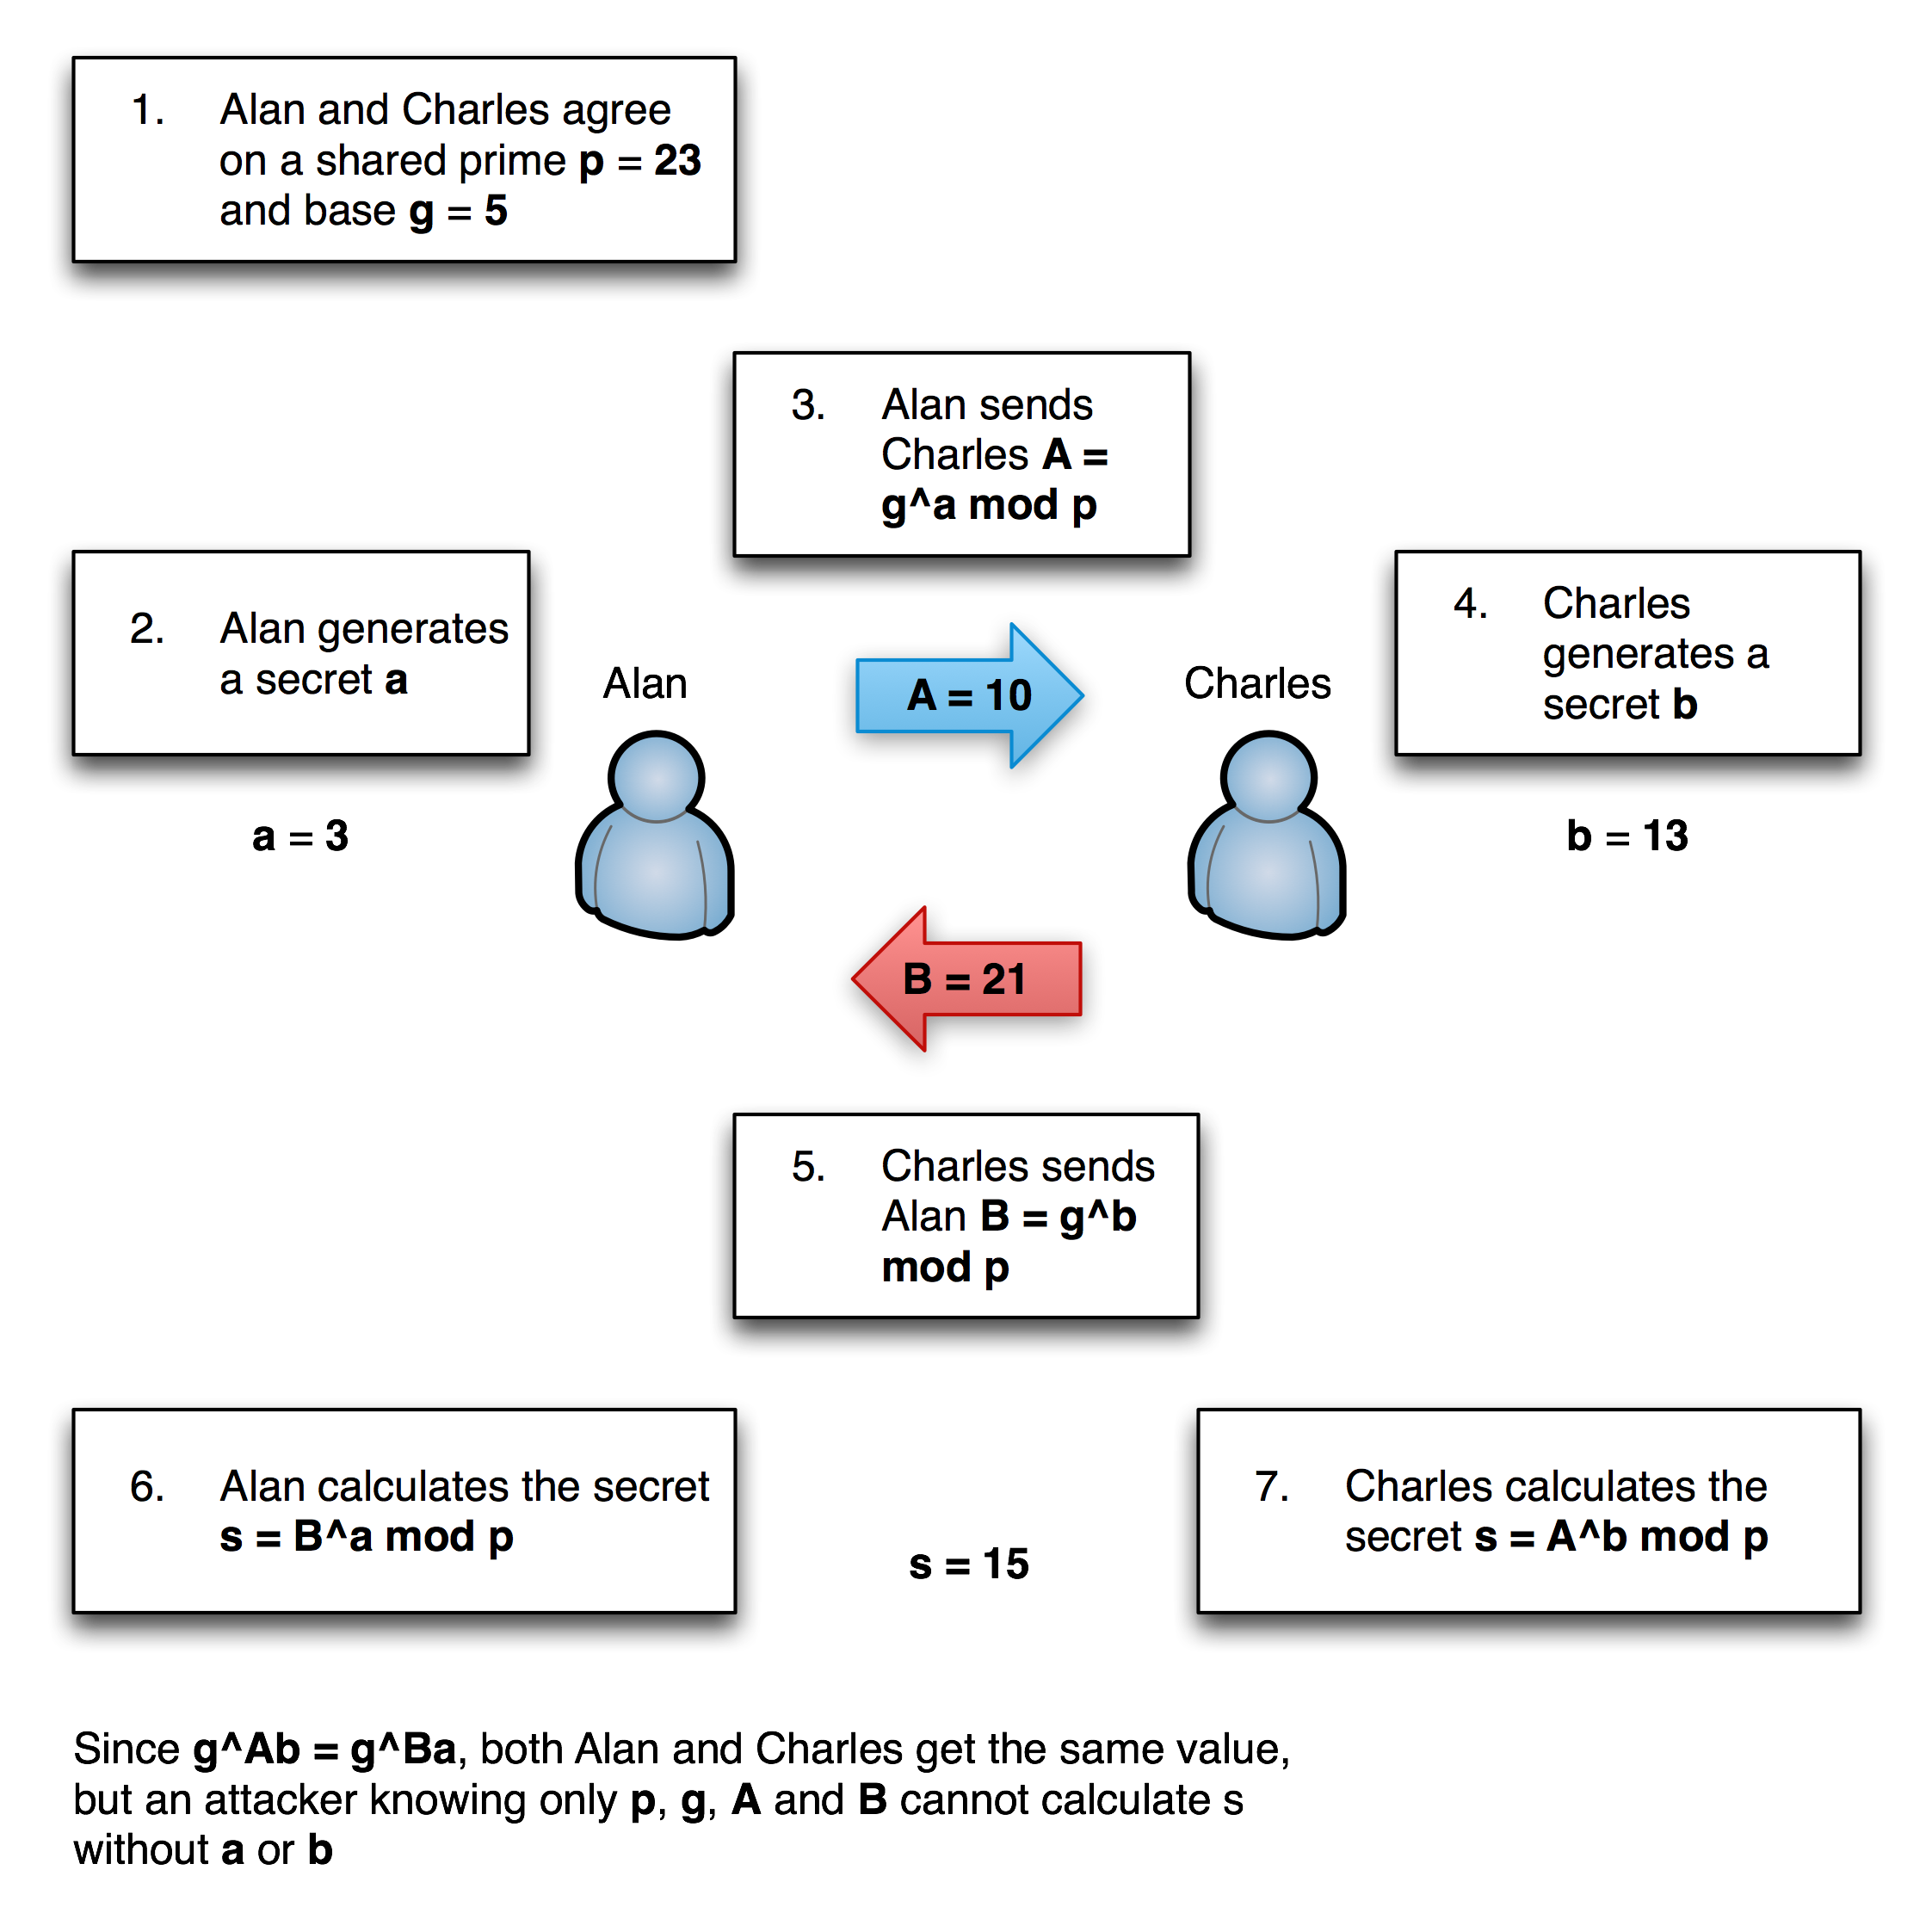
\includegraphics[width=\linewidth]{key-exchange}
\caption{Diffie-Hellman Key Exchange}
\label{key-exchange}
\end{figure}

Public key cryptography has seen a number of advancements based on these early discoveries, with the development of an asymmetric key encryption method based on Diffie-Hellman named after its creator \citet*{ElGamal:1985p529}. Various mathematical problems have been used in the development of newer crypto systems, with increasing complexity such as the use of  elliptic curve cryptography in \cite{Miller:1986p2966} and \cite{Koblitz:1987p3109}, probabilistic functions in \cite{Paillier:1999p3152} and to address weaknesses in \cite{Cramer:1998p3186}.

Public key cryptography is the foundation of Internet based cryptography and anonymous networks. Conventional methods of sharing secret keys by courier or post are costly and negate the benefits provided by a digital network. Although \cite{Baran:1964p384} proposed encryption for usage in digital communications, citing benefits such as tamper resistance, message secrecy and resistance to traffic analysis. This system was never implemented.

Early work in encrypted Internet communications includes the Secure Network Programming (SNP) applications programming interface (API) \citep{Woo:1994p2532}. This was simply a framework providing numerous encryption, signing and authentication methods. The Secure Sockets Layer (SSL) is an encryption layer which provided end to end communications secrecy on the Internet \citep{website:SSL}. It makes use of public key cryptography to ensure secrecy.

This proposed standard went through a number of revisions, with early versions suffering security flaws \citep{Wagner:1996p385}. SSL is now known as Transport Layer Security, with the latest version 1.2 being released August 2008 \citep{website:TLS}. TLS addresses some issues in SSL and provides a number of enhancements, but is not compatible.

The Hypertext Transfer Protocol Secure (HTTPS) makes use of both SSL and TLS and the Hypertext Transfer Protocol (HTTP) to provide encryption and secure identification when visiting websites \citep{website:HTTPS}. This is also the protocol used by Tor.

\section{Anonymous and Censorship Resistant Networks}

The first anonymous network system was proposed in \cite{Chaum:1981p296}. This proposal included the use of public key cryptography and a centrally located server known as a ‘mix’. By wrapping the information and address of a destination in a message and encrypting it with the mix’s public key, only the mix system is able to read the message.

\begin{figure}[H]
\center 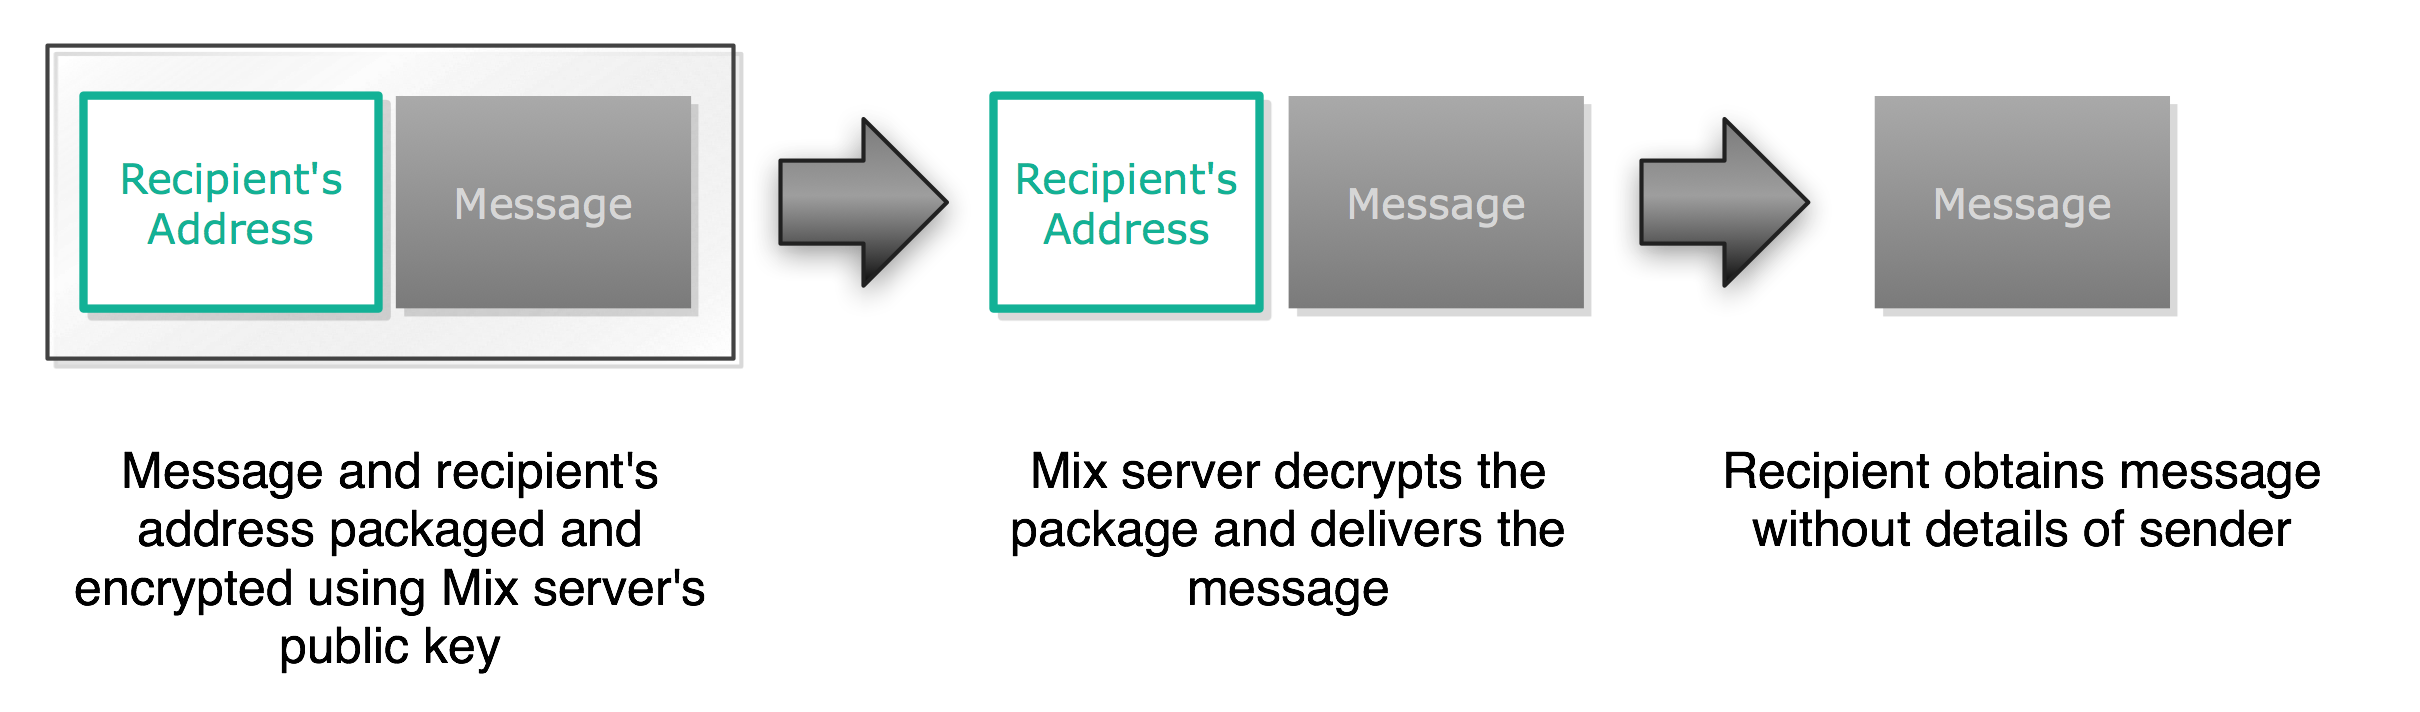
\includegraphics[width=\linewidth]{chaums-mix-network}
\caption{Chaum's Mix Network}
\label{chaums-mix-network}
\end{figure}

The mix system then delivers the message to its destination without passing any information on about the sender. Because the destination system only communicates with the mix server, it has no information available about the sender in which to make a positive identification.

Since this proposal, many networks have been developed that provide features such as anonymity and censorship resistance. The proposed systems differ with regard to the motivation behind providing anonymity. Like cryptography, an arms race between anonymous network designers and those discovering attacks has motivated development of iterative refinements in response to weaknesses.

Many early systems were designed to provide anonymous email delivery, these include Babel \citep{Gulcu:1996p1662}, Mixminion \citep{Danezis:2003p1616} as well as Nym servers \citep{Mazieres:1998p4560} and two commercial offerings Underhill and NymBaron. One of the earliest anonymous remailers anon.penet.fi was created by Johan Helsingius in 1993, but was shutdown in 1996 due to a combination of legal pressure and an inability to provide true anonymity \cite{Danezis:2008p346}.

The need for anonymous networks to resist attack and node failure led to the development of various robust mix networks such as \citep{Waidner:1989p5870}, \citep{Park:1994p5051}, (Kilian  Sako, 1995), \citep{Ogata:1997p5083}, \citep{Abe:1998p1898}, \citep{Jakobsson:1998p5137} and (Desmedt and Kurosawa, 2000).  An avenue of research in robust mix networks is universal re-encryption described in \citep{Fairbrother:2005p5357}, \citep{Lu:2005p5387}, (Lu et al., 2006) and \citep{Gomukiewicz:2004p294}.

The problem of mathematically provable anonymity is a difficult one, and many proposals have been developed \citep{Chaum:1988p5869}, \citep{Rackoff:1993p5817}, \citep{Kesdogan:1998p2027}, \citep{Jakobsson:1999p2008} \cite{Neff:2001p2068}, \cite{Furukawa:2001p5158}, \citep{Golle:2004p5204}, \citep{Gomukiewicz:2003p5816}, \citep{Berman:2004p303}, \citep{Golle:2004p5204}, \citep{Adida:2007p5205}, \citep{Klonowski:2005p5379}, \citep{Nguyen:2008p3837}. In practice however, strong provable anonymity incurs a great deal of performance overhead and has not seen wide usage \citep{Danezis:2008p346}.

Attempts to make provable anonymity more attractive by increasing performance includes Flash mixing, a scheme for more efficient anonymity using mixes \citep{Jakobsson:1999p2008}.

Stop and Go Mixes which provide probabilistic anonymity and don’t require a confirmed identity to participate \citep{Kesdogan:1998p2027}.

Discouraging network operators from divulging known identities is a feature of intentionally fragile mix networks such as \citep{Reiter:2004p5868} and (Golle et al., 2006). These networks are designed to make the process of tracing a single message damaging to the system or its property of anonymity, making compulsion potentially expensive.

\cite{Jakobsson:2002p5815} \cite{Goel:2003p5871}

The practice of steganography allows for the hiding of messages within existing mechanisms, which provides some measure of anonymity and censorship resistance by making messages undetectable to observers. Steganography has been proposed as a way of providing censorship resistance in (Feamster et al., 2002), (Feamster et al., 2003). The use of covering traffic and rerouting of messages to complicate traffic analysis is discovered in \citep{Venkatraman:1995p6008}, (Timmerman, 1997), (Timmerman, 1999), (Guan et al., 2001) and (Newman et al., 2003).

Most anonymous and censorship resistant networks provide means for using well established Internet protocols in an anonymous manner, some however have provided standalone means of publishing information anonymously. These include Freedom (Boucher et al., 2000) and Freenet (Clarke et al., 2001) which provides a network for publishing with anonymity for both authors and readers by collectively sharing storage.

The success of peer to peer (p2p) systems such as Bittorrent and Kazaa has inspired the development of p2p anonymous networks such as MorphMix \citep{Rennhard:2002p4559}, Tarzan (Freedman, 2002) and P5 (Sherwood et al., 2005).

Private Information Retrieval:

(Kissner et al., 2004) (Sassaman et al., 2005) (Danezis and Diaz, 2006) (Ostrovsky and Keith, 2007) (Bethencourt et al., 2009)

Some anonymous networks have been developed with the explicit goal of censorship resistance, these include aChord (Hazel and Wiley, 2002), gnuNet (Hazel and Wiley, 2002), (Anderson, 1996), (Serjantov, 2002) and (Clayton et al., 2006)

\subsection{The Second Generation Onion Router(Tor)}

Tor was first described in Tor: The Second-Generation Onion Router (Dingledine et al., 2004). This new generation of onion router was designed with a number of defences for common traffic analysis attacks and weaknesses in previous proposals. A number of these design decisions make Tor a more attractive system for the general user and have encouraged wider deployment.

The Tor network, like the Mix-Net proposed in Chaum (1981) uses public key encryption and cascades of servers to ensure message anonymity. In Tor these mixes are known as ‘relays’. Relays that allow connections directly from Tor clients are known as ‘bridges’ and relays that deliver messages from the frontier of the Tor network are known as ‘exit nodes’. Figure \ref{tor-network} shows how a client connects to the Tor network.

\begin{figure}[H]
\center 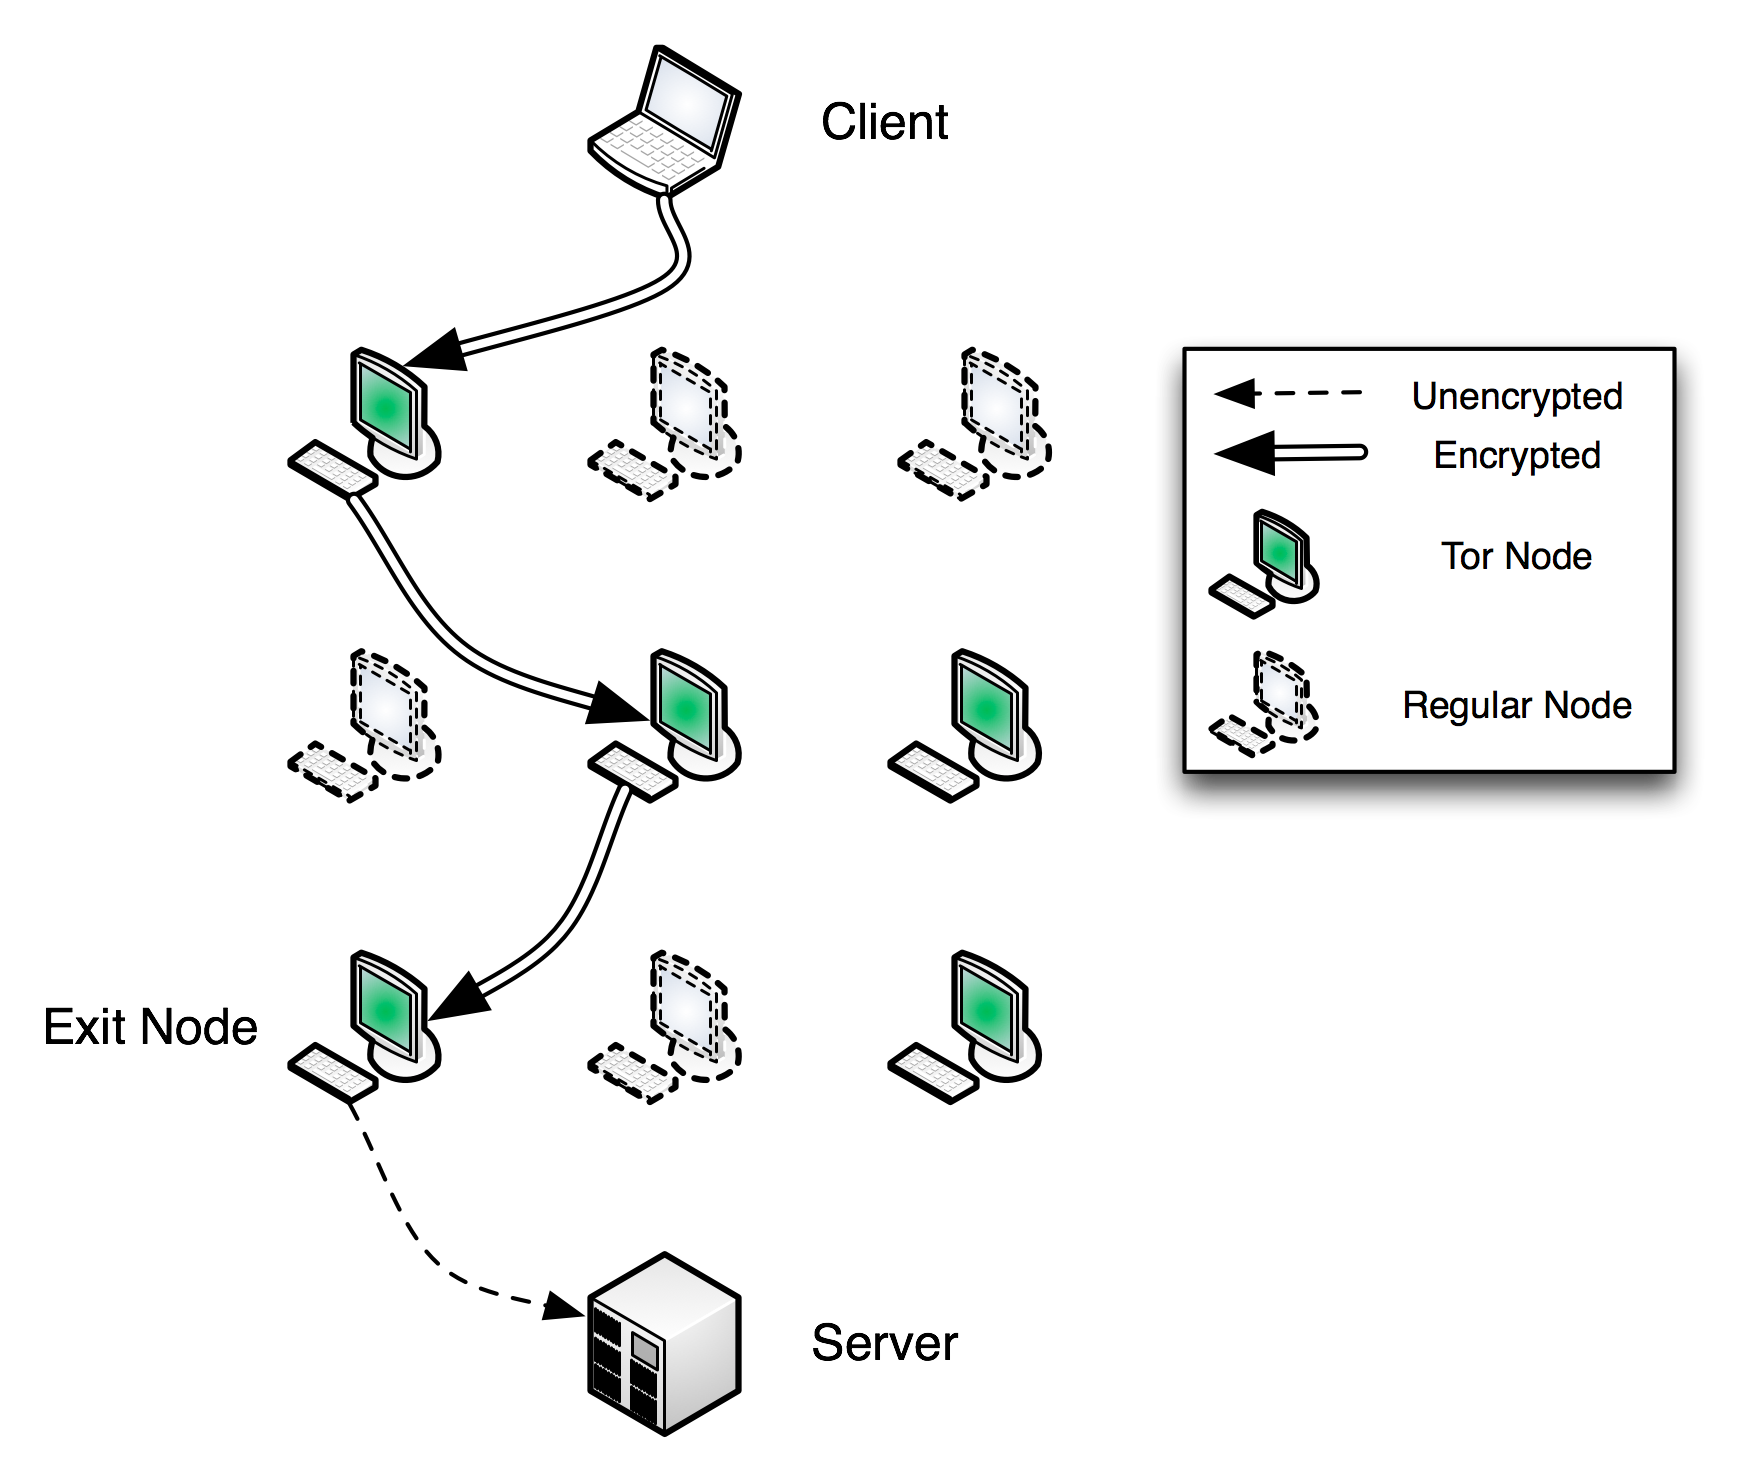
\includegraphics[width=\linewidth]{tor-network-diagram}
\caption{The Tor Network}
\label{tor-network}
\end{figure}

When a relay joins the Tor network, it trades symmetric cipher keys with its neighbours using public key cryptography. These keys are used to encrypt communications and are destroyed when the session is closed to prevent replay attacks.

After it was noticed that Tor was being used to circumvent censorship as well as for anonymity, a proposal was developed to improve its blocking resistance \citep{Dingledine:2008p1542}. Many of the suggestions in this proposal have been implemented, but many still remain.

Apart from traffic analysis attacks, Tor nodes have been run by hostile parties to capture private information (Goodin, 2007)

\section{Traffic Analysis}

The development of radio led to a great change in the theatre of war, giving generals almost instant control over their armies. This proved to be a double edged sword, the broadcast nature of radio communications made it easier for enemies to intercept communications. While encryption methods were developed to provide resistance against eavesdropping, the patterns exhibited by radio signals allowed for the identification of the communicators, the language they used or the location they resided \cite{Kahn:1967p1005}.

When considering the use of traffic analysis for Internet communications, three  techniques are used. These are: exact matching, heuristic matching and machine learning \citep{Zhang:2009p1188}.

Exact matching techniques recognise properties of communications that mirror known protocols and communication patterns. This might include the port an application uses or the format of its payload. Since anonymous networks typically use encryption and avoid using known or published communication patterns, these kind of attacks are not applicable.

Heuristic matching looks for patterns in conversations to determine communications patterns and infer relationships. Finally, machine learning involves the use of statistics to train computer algorithms to classify traffic. Both heuristic and machine matching techniques are suitable for traffic analysis of anonymous networks because they do not rely on analysing the content of messages.

\subsection{Heuristic Techniques}

The increasing burden of peer to peer (P2P) applications on campus networks, and their shift to encryption motivated the development of heuristics based techniques for identifying P2P traffic. Early techniques include identifying known properties of P2P networks such as often communicating using both the UDP and TCP protocols simultaneously and using a solitary connection to transfer high volumes \citep{Karagiannis:2004p6400}. This paper also reduced the number of false positives by eliminating packets that matched known communications protocols.

Similar techniques have been developed in \citep{Perenyi:2006p6325} and \citep{John:2008p1376}, both of which attempt to improve matching accuracy by expanding the scope of matching parameters and eliminating more false positives. In \cite{Oneil:2004p6451} the same heuristics are used to identify P2P nodes before applying a secondary heuristic to identify ‘supernodes’ which are a subset of all P2P nodes.

Classifying traffic based on system roles is a key feature of the technique that appears in BLINC: Multilevel Traffic Classification in the Dark \citep{Karagiannis:2005p6359}. By analyzing communications at the host level then at increasing levels of granularity, a greater level of accuracy is achieved.

The use of Traffic Dispersion Graphs or TDGs to identify P2P traffic appears in \cite{Iliofotou:2008p6373} and \cite{Iliofotou:2009p6461}. Once traffic flows are represented in a TDG, mathematical properties of the flow can be analyzed to make positive identifications.

Viruses have also posed a problem for network administrators, often over-utilizing network resources and using the network to infect new machines. A technique for identifying various worms was proposed in \cite{Lazarevic:2003p6450}.

\subsection{Machine Learning Techniques}

\subsubsection{Expectation-Maximisation}

The first use of machine learning to categorise traffic flows appears in \cite{McGregor:2004p3826}. A detailed analysis of the attributes that can be used for machine learning and an attempt at coarse grained classification using an Expectation-Maximisation (EM) algorithm are demonstrated. The same technique is also demonstrated in \cite{Soule:2004p3817} using histograms for finer grained classification. The EM algorithm is again used in \cite{Zander:2005p6212} and \cite{Erman:2006p3825}, with the latter also comparing this algorithm favourably against a Naïve Bayes classifier.

\subsubsection{Naïve Bayes}

\cite{Moore:2005p3827} use a supervised Naïve Bayes to classify traffic flows that have previously been sorted into groups by analysing the flow content. This paper focuses on many of the most commonly used Internet protocols while \cite{Bonfiglio:2007p6453} uses the technique for identifying traffic belonging to the commercial Skype application.

\cite{Herrmann:2009p1189} use Bayesian networks to fingerprint visited websites accessed through Privacy Enhancing Technologies (PET), including Tor. This technique performed poorly when applied to the Tor network, but it suggests that Tor traffic has particular characteristics that distinguish it from many existing PETs. It makes a particularly useful observation: “The most frequent packet sizes in the Tor traffic dumps are, in descending order, 1500, −52, −638, 52, 638 and 1150 bytes, accounting for 87.6 \% of all Tor packets.”

\subsubsection{Hidden Markov Model}

Hidden Markov Models are first used as a traffic analysis technique in HMM profiles for network traffic classification \citep{Wright:2004p3860}. The primary identification characteristics for use with this algorithm are packet size and inter-packet arrival times. With refinement this algorithm is used with increasing accuracy in \cite{Wright:2006p322} and \cite{Dainotti:2008p1435}. HMMs are also used in \cite{Bernaille:2005p6205} to discover distinguishing characteristics of traffic flows, rather than specifically as a classifier.

\subsubsection{Clustering}

Clustering algorithms group observations into subsets based on similar characteristics. They have been used in a number of traffic classification techniques with the K-Means clustering technique being the most prominent. K-Means cluster analysis appears in Bernaille et al. (2006), \cite{Erman:2007p3764}, \cite{Erman:2007p6206}. The use of the Density Based Spatial Clustering of Applications with Noise (DBSCAN) algorithm appears in \cite{Erman:2006p3766}, alongside K-Means and Autoscan algorithms.

\subsubsection{Other Techniques}

Other algorithms used for traffic classification include Nearest Neighbour and  Linear Discriminant Analysis \citep{Roughan:2004p3823}, Normalized Threshold \citep{Crotti:2007p3824}. The use of the Gaussian Mixture Model to identify applications and identities inside SSH tunnels was demonstrated in \cite{Dusi:2008p6254}.

\subsubsection{Comparing Techniques}

It is difficult to say what machine learning technique is the most effective as no consensus has been reached, the literature covers a wide variety of techniques each with vastly different goals and no two techniques can be directly compared as the data used for analysis has not been disclosed \citep{Kim:2007p3867}. However some attempt has been made at comparison in \cite{Williams:2006p3849} which suggests that the C4.5 algorithm has the greatest performance and accuracy when compared to a number of Bayesian algorithms. \cite{Mohd:2009p6484} compares thirty machine learning algorithms  to find random tree, IBI, IBK and random forest algorithms obtaining the greatest classification accuracy.

An excellent meta study on traffic analysis techniques is presented in \cite{Nguyen:2008p3837}. This paper compares many of the published papers, the techniques used, criteria analysed and how effectively they meet stated goals.

\chapter{Theoretical Framework}

The proposed research will use a methodology typical of machine learning traffic analysis papers, substituting data captured from a controlled simulation in place of live network captures. 

The experiment will be conducted in two phases, the first being a data collection phase. The second phase will include a quasi experimental methodology which may include data manipulation techniques to prepare the collected data and a comparison of various heuristics and machine learning based traffic analysis to classify the collected data.

\section{Assumptions}

It is assumed that the usage patterns exhibited by individual users will be smaller than the communications characteristics that will lead to the identification of anonymous and censorship resistant networks. Thus there is no need to obtain a large sample of regular network traffic from varying user profiles.

As of the current implementation, Tor network traffic is readily distinguishable by looking at the handshake packets. It is likely that this weakness will be addressed in a future version of the Tor protocol as it is recognised as a design goal in \cite{Dingledine:2008p1542}. For this reason, this proposal focuses on traffic analysis techniques that are content agnostic.

\section{Variables}

The data capturing stage will be affected by a number of variables that will influence the accuracy of the chosen matching algorithms.

\subsection{System Performance}

Packet latency is highly dependent on the performance of a computer system  and how busy it is. Performance related variables include:

\begin{itemize*}
\item CPU speed and number of cores
\item RAM speed and amount
\item Performance of integrated components, system bus etc.
\item Hard disk size, access time and throughput
\item Installed and running applications
\item System configuration
\end{itemize*}

To remedy this, the systems used to simulate the Tor network should be made uniform. This means an identical hardware and software configuration for all systems in the simulation network.

In addition it is noted that system performance can degrade over time due to both memory and hard disk fragmentation. This can be avoided by running the simulations in a virtualisation environment that support snapshots, rolling back to a known configuration point after each test.

\subsection{Network Performance}

Like system performance, latency is also dependent on the quality of the network. Network switching equipment has limited resources for routing packets and competing network traffic can introduce unpredictable delays into the sampled data. 

Isolating the test network from the wide area network or Internet can help reduce these variables significantly as well as ensuring that all unnecessary network related software is uninstalled or disabled.

\subsection{Application Protocol}

Tor provides communications facilities to a number of Internet enabled applications by providing an interface using the SOCKS protocol. This means that the Tor network can proxy regular web browsing, email or any other TCP based communication protocol. Each of these application protocols have their own distinguishing communications characteristics which will influence the matching algorithm. It is not yet clear how transparent the Tor network will be regarding these characteristics and thus, for the purposes of classification a single protocol should be chosen.

\subsection{Quality of the Anonymous Network}

An individual connection to the Tor network traverses a number of nodes to create a circuit, these individual nodes can vary wildly in the following ways:

\begin{itemize*}
\item The geographic location of each node
\item Network bandwidth and latency
\item System load
\item Network load
\item Configuration
\end{itemize*}

Each communication session established creates a new circuit, of which the nodes that comprise this circuit are chosen randomly.

For testing purposes, the Tor network can be simulated on a small network. This will eliminate a lot of the variability that comes from monitoring the real Tor network. Factors that affect the quality of the network can be controlled by limiting the number of competing network applications, controlling the number of running Tor instances and ensuring a consistent configuration across all nodes.

\subsection{Caching}

Both web browsers and web servers are designed for high performance and often cache requests so that they can be delivered faster in the future. While this is a normal part of communications traffic and should be considered, it is important that uncached and cached requests appear in equal volume in all experiments. Manually flushing the cache or rolling back to a known virtual machine snapshot between each simulation can ensure this outcome.

\chapter{Materials and Methods}

\section{Equipment Requirements}

The following list describes computer systems and hardware required to run the data capture simulations:

\begin{itemize*}
\item 1 Computer system running web browser and Tor
\item 1 Computer running packet sniffing software
\item N Computer systems running Tor, configured as bridges
\item 1 Computer running web server and Tor directory server
\item Cat 5 cable to connect all computer systems
\item Network Hub or Switch capable of disabling ‘learning’ \citep{website:hub-reference}
\end{itemize*}

The computer systems running Tor bridges represent the simulation network. Although it is feasible to have a single system representing the simulation network the combined system load may be too great and introduce  excessive latency.

Packet capture is a performance intensive application, 1 machine should be reserved for this application. It must include adequate disk space, preferably of a high speed. 

The required software includes:

\begin{itemize*}
\item Virtualisation software
\item Web browser
\item Tor
\item Packet capture software
\end{itemize*}

\subsection{Procedure}

\subsubsection{Phase 1}

\paragraph{Hardware Configuration}

All systems will be configured and connected to the same isolated network through the hub as shown in Figure \ref{physical-setup}.

\begin{figure}[h]
\center 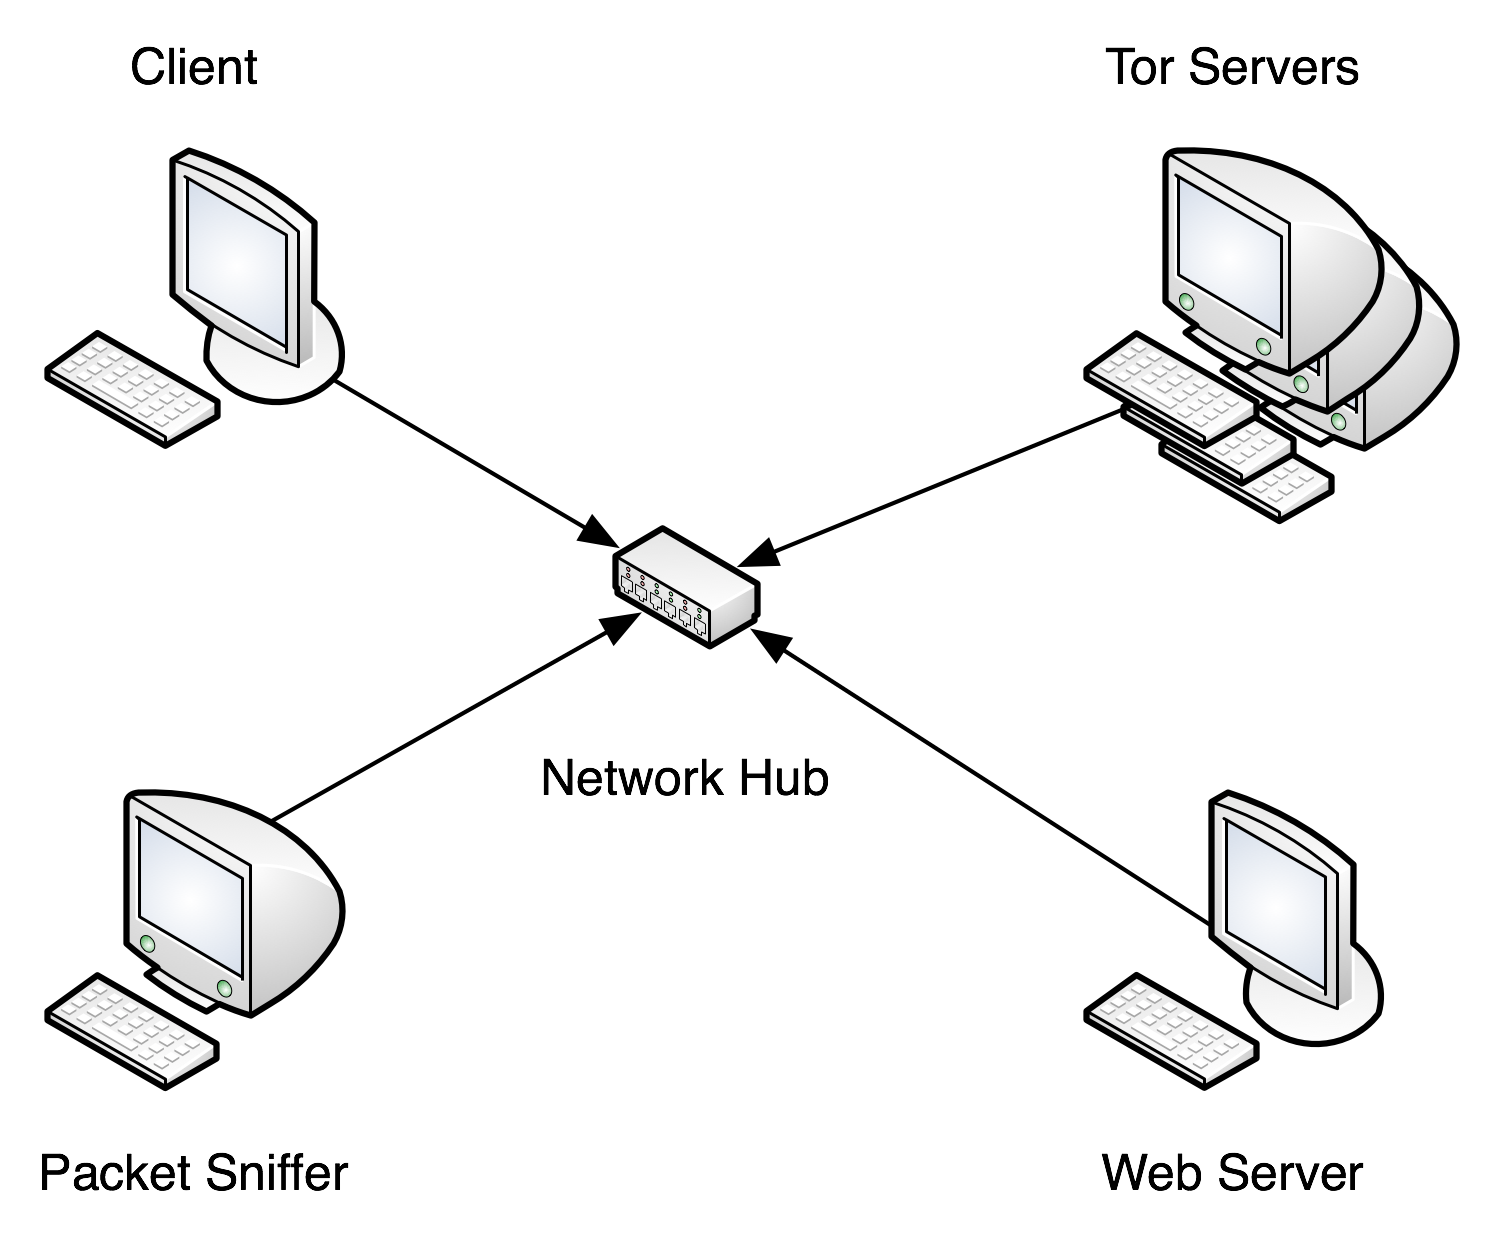
\includegraphics[scale=0.8]{physical-setup}
\caption{Physical Setup}
\label{physical-setup}
\end{figure}

\paragraph{Software Configuration}

Software is installed and configured on all machines. The simulation network is configured to use the private Tor directory server rather than the public ones specified by default.

The packet sniffer is configured to capture only the packets relevant for each data set.

Figure \ref{network-diagram} shows the placement of applications and relevant data flows.

\begin{figure}
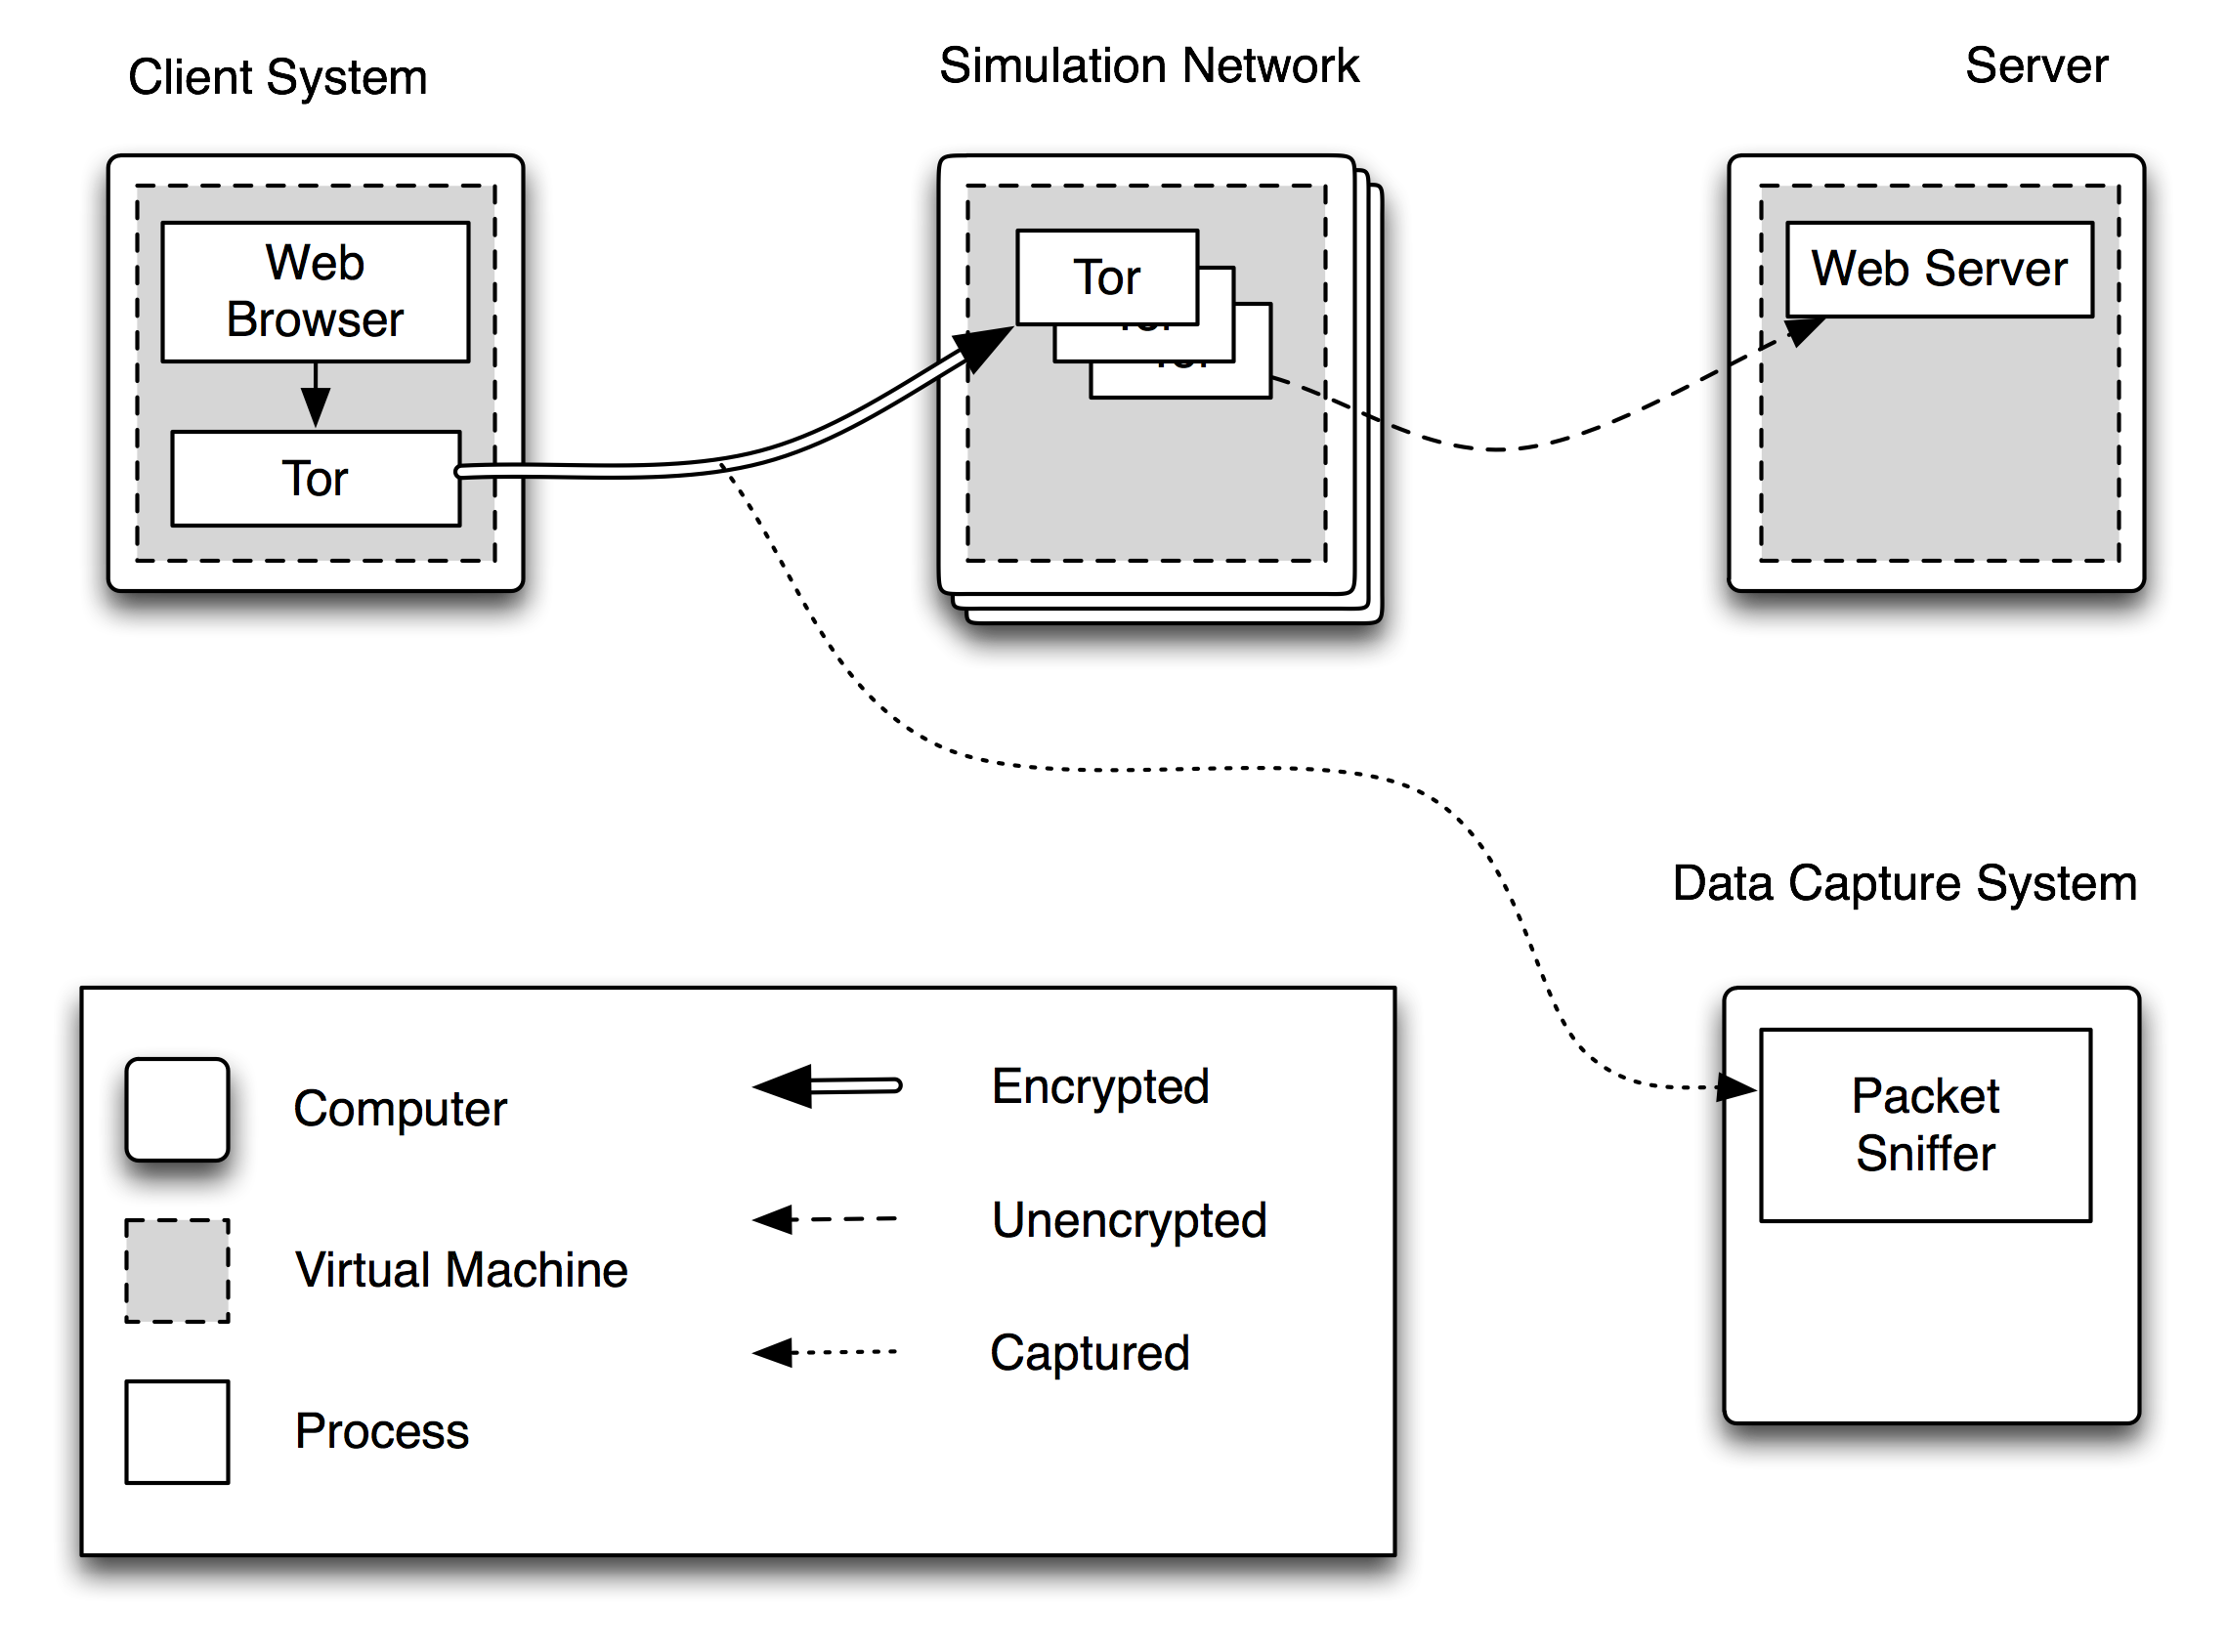
\includegraphics[width=\linewidth]{network-diagram}
\caption{Network Diagram}
\label{network-diagram}
\end{figure}

\paragraph{Simulations}

A number of simulations will be performed. The web server 

\paragraph{Data Capture}

Three sets of data must be collected, and kept separate. The first set is a sample that is known to belong to the anonymous networks in question. To capture this the software will be configured to communicate using known parameters. It will also be ensured that no other applications are communicating using these parameters that may pollute the data set.

This first set of data can be partitioned to make the second set, which will be used to confirm the false negative rate of the matching technique.

The third set of data must constitute traffic that is known to not contain any traffic from the networks being catalogues. This data set will be used to confirm the rate of false positives.

\subsection{Phase 2}

\subsubsection{Data Preparation}

The captured data will be in the data file format used by the capture software. For analysis the most relevant information needs to be retrieved from the data files and prepared in a suitable format for the matching algorithm.

\paragraph{Analysis}

The training data set will be supplied to the algorithm for training purposes. Once training is complete, this algorithm can be tested against the confirmation data set to obtain the rate of false negatives. The regular traffic will be used to determine the false positive rate. This allows the construction of the Receiver Operating Characteristic (ROC) curve, a measurement of the performance of the matching algorithm.

\section{Limitations}

The process has been designed with a goal to minimising variables that may affect matching performance - this is unusual for traffic analysis papers which typically sample real world traffic in large volumes. In the case of a machine learning technique, this may bias the chosen algorithm against real world data, making it impractical for any real world use.

\section{Schedule}

\begin{tabular}{llr}
\toprule
Activity & Duration & Date \\
\midrule
Phase 1 \\
1 - Setup hardware & 1 week \\
2 - Configure simulations & 1 week \\
3 - Run simulations/data capture & 4 weeks \\
Phase 2 \\
1 - Data preparation & 4 week \\
2 - Algorithm training and selection & 8 weeks \\
Document final results and writeup & * \\
\midrule
Thesis submission & & December 4th, 2011 \\
\bottomrule
\end{tabular}

\bibliography{papers,websites}

\end{document}

% vim: fdm=syntax
